\documentclass[twoside,11pt]{article}

% ? Specify used packages
\usepackage{graphicx}        %  Use this one for final production.
% \usepackage[draft]{graphicx} %  Use this one for drafting.
% ? End of specify used packages

\pagestyle{myheadings}

% -----------------------------------------------------------------------------
% ? Document identification

% Fixed part
\newcommand{\stardoccategory}  {Starlink User Note}
\newcommand{\stardocinitials}  {SUN}
\newcommand{\stardocsource}    {sun\stardocnumber}

% Variable part - replace [xxx] as appropriate.
\newcommand{\stardocnumber}    {214.32}
\newcommand{\stardocauthors}   {Peter W. Draper, 
                                Norman Gray, 
                                David S. Berry \& 
                                Mark Taylor }
\newcommand{\stardocdate}      {14th November 2007}
\newcommand{\stardoctitle}     {GAIA -- 
                                Graphical Astronomy and Image Analysis Tool}
\newcommand{\stardocversion}   {4.1-0}
\newcommand{\stardocmanual}    {User's Manual}

\newcommand{\stardocabstract} {GAIA is an image and data-cube display 
and analysis tool for astronomy. It provides the usual facilities of image
display tools, plus more astronomically useful ones such as aperture \&
optimal photometry, contouring, source detection, surface photometry,
arbitrary region analysis, celestial coordinate readout, calibration
and modification, grid overlays, blink comparison, defect patching and
the ability to query on-line (WWW) catalogues and image servers. It can 
also display slices from data-cubes, extract and visualise spectra as 
well as perform full 3D rendering.}

% ? End of document identification
% -----------------------------------------------------------------------------

% +
%  Name:
%     sun.tex
%
%  Purpose:
%     Template for Starlink User Note (SUN) documents.
%     Refer to SUN/199
%
%  Authors:
%     AJC: A.J.Chipperfield (Starlink, RAL)
%     BLY: M.J.Bly (Starlink, RAL)
%     PWD: Peter W. Draper (Starlink, Durham University)
%
%  History:
%     17-JAN-1996 (AJC):
%        Original with hypertext macros, based on MDL plain originals.
%     16-JUN-1997 (BLY):
%        Adapted for LaTeX2e.
%        Added picture commands.
%     13-AUG-1998 (PWD):
%        Converted for use with LaTeX2HTML version 98.2 and
%        Star2HTML version 1.3.
%     {Add further history here}
%
% -

\newcommand{\stardocname}{\stardocinitials /\stardocnumber}
\markboth{\stardocname}{\stardocname}
\setlength{\textwidth}{160mm}
\setlength{\textheight}{230mm}
\setlength{\topmargin}{-2mm}
\setlength{\oddsidemargin}{0mm}
\setlength{\evensidemargin}{0mm}
\setlength{\parindent}{0mm}
\setlength{\parskip}{\medskipamount}
\setlength{\unitlength}{1mm}

% -----------------------------------------------------------------------------
%  Hypertext definitions.
%  ======================
%  These are used by the LaTeX2HTML translator in conjunction with star2html.

%  Comment.sty: version 2.0, 19 June 1992
%  Selectively in/exclude pieces of text.
%
%  Author
%    Victor Eijkhout                                      <eijkhout@cs.utk.edu>
%    Department of Computer Science
%    University Tennessee at Knoxville
%    104 Ayres Hall
%    Knoxville, TN 37996
%    USA

%  Do not remove the %begin{latexonly} and %end{latexonly} lines (used by
%  LaTeX2HTML to signify text it shouldn't process).
%begin{latexonly}
\makeatletter
\def\makeinnocent#1{\catcode`#1=12 }
\def\csarg#1#2{\expandafter#1\csname#2\endcsname}

\def\ThrowAwayComment#1{\begingroup
    \def\CurrentComment{#1}%
    \let\do\makeinnocent \dospecials
    \makeinnocent\^^L% and whatever other special cases
    \endlinechar`\^^M \catcode`\^^M=12 \xComment}
{\catcode`\^^M=12 \endlinechar=-1 %
 \gdef\xComment#1^^M{\def\test{#1}
      \csarg\ifx{PlainEnd\CurrentComment Test}\test
          \let\html@next\endgroup
      \else \csarg\ifx{LaLaEnd\CurrentComment Test}\test
            \edef\html@next{\endgroup\noexpand\end{\CurrentComment}}
      \else \let\html@next\xComment
      \fi \fi \html@next}
}
\makeatother

\def\includecomment
 #1{\expandafter\def\csname#1\endcsname{}%
    \expandafter\def\csname end#1\endcsname{}}
\def\excludecomment
 #1{\expandafter\def\csname#1\endcsname{\ThrowAwayComment{#1}}%
    {\escapechar=-1\relax
     \csarg\xdef{PlainEnd#1Test}{\string\\end#1}%
     \csarg\xdef{LaLaEnd#1Test}{\string\\end\string\{#1\string\}}%
    }}

%  Define environments that ignore their contents.
\excludecomment{comment}
\excludecomment{rawhtml}
\excludecomment{htmlonly}

%  Hypertext commands etc. This is a condensed version of the html.sty
%  file supplied with LaTeX2HTML by: Nikos Drakos <nikos@cbl.leeds.ac.uk> &
%  Jelle van Zeijl <jvzeijl@isou17.estec.esa.nl>. The LaTeX2HTML documentation
%  should be consulted about all commands (and the environments defined above)
%  except \xref and \xlabel which are Starlink specific.

\newcommand{\htmladdnormallinkfoot}[2]{#1\footnote{#2}}
\newcommand{\htmladdnormallink}[2]{#1}
\newcommand{\htmladdimg}[1]{}
\newcommand{\hyperref}[4]{#2\ref{#4}#3}
\newcommand{\htmlref}[2]{#1}
\newcommand{\htmlimage}[1]{}
\newcommand{\htmladdtonavigation}[1]{}

\newenvironment{latexonly}{}{}
\newcommand{\latex}[1]{#1}
\newcommand{\html}[1]{}
\newcommand{\latexhtml}[2]{#1}
\newcommand{\HTMLcode}[2][]{}

%  Starlink cross-references and labels.
\newcommand{\xref}[3]{#1}
\newcommand{\xlabel}[1]{}

%  LaTeX2HTML symbol.
\newcommand{\latextohtml}{\LaTeX2\texttt{HTML}}

%  Define command to re-centre underscore for Latex and leave as normal
%  for HTML (severe problems with \_ in tabbing environments and \_\_
%  generally otherwise).
\renewcommand{\_}{\texttt{\symbol{95}}}

% -----------------------------------------------------------------------------
%  Debugging.
%  =========
%  Remove % on the following to debug links in the HTML version using Latex.

% \newcommand{\hotlink}[2]{\fbox{\begin{tabular}[t]{@{}c@{}}#1\\\hline{\footnotesize #2}\end{tabular}}}
% \renewcommand{\htmladdnormallinkfoot}[2]{\hotlink{#1}{#2}}
% \renewcommand{\htmladdnormallink}[2]{\hotlink{#1}{#2}}
% \renewcommand{\hyperref}[4]{\hotlink{#1}{\S\ref{#4}}}
% \renewcommand{\htmlref}[2]{\hotlink{#1}{\S\ref{#2}}}
% \renewcommand{\xref}[3]{\hotlink{#1}{#2 -- #3}}
%end{latexonly}
% -----------------------------------------------------------------------------
% ? Document specific \newcommand or \newenvironment commands.
\newcommand{\mytt}[1]{{\texttt{#1}}}
\newcommand{\mybold}[1]{{\textbf{#1}}}
% ? End of document specific commands
% -----------------------------------------------------------------------------
%  Title Page.
%  ===========
\renewcommand{\thepage}{\roman{page}}
\begin{document}
\thispagestyle{empty}

%  Latex document header.
%  ======================
\begin{latexonly}
   CCLRC / \textsc{Rutherford Appleton Laboratory} \hfill \textbf{\stardocname}\\
   {\large Particle Physics \& Astronomy Research Council}\\
   {\large Starlink Project\\}
   {\large \stardoccategory\ \stardocnumber}
   \begin{flushright}
   \stardocauthors\\
   \stardocdate
   \end{flushright}
   \vspace{-4mm}
   \rule{\textwidth}{0.5mm}
   \vspace{5mm}
   \begin{center}
   {\Large\textbf{\stardoctitle \\ [2.5ex]}}
   \vspace{5mm}
% ? Add picture here if required for the LaTeX version.
   \includegraphics[totalheight=5in]{sun214fig.ps}
% ? End of picture
   \end{center}

% ? Heading for abstract if used.
   \begin{center}
      {\Large\textbf{Abstract}}
   \end{center}
% ? End of heading for abstract.
\end{latexonly}

%  HTML documentation header.
%  ==========================
\begin{htmlonly}
   \xlabel{}
   \begin{rawhtml} <H1> <FONT COLOR="#000099">\end{rawhtml}
   \begin{center}
      \stardoctitle
    \end{center}
   \begin{rawhtml} </FONT></H1> \end{rawhtml}

% ? Add picture here if required.
   \begin{center}
   \htmladdimg{sun214.jpg}
   \end{center}
% ? End of picture
   \begin{rawhtml} <P> <I> \end{rawhtml}
   \stardoccategory\ \stardocnumber \\
   \stardocauthors \\
   \stardocdate
   \begin{rawhtml} </I> </P> <H3> \end{rawhtml}
      \htmladdnormallink{CCLRC / Rutherford Appleton Laboratory}
                        {http://www.cclrc.ac.uk} \\
      \htmladdnormallink{Particle Physics \& Astronomy Research Council}
                        {http://www.pparc.ac.uk} \\
   \begin{rawhtml} </H3> <H2> \end{rawhtml}
      \htmladdnormallink{Starlink Project}{http://www.starlink.ac.uk/}
   \begin{rawhtml} </H2> \end{rawhtml}
   \htmladdnormallink{\htmladdimg{source.gif} Retrieve hardcopy}
      {http://www.starlink.ac.uk/cgi-bin/hcserver?\stardocsource}\\

%  HTML document table of contents.
%  ================================
%  Add table of contents header and a navigation button to return to this
%  point in the document (this should always go before the abstract \section).
  \label{stardoccontents}
  \begin{rawhtml}
    <HR>
    <H2>Contents</H2>
  \end{rawhtml}
  \htmladdtonavigation{\htmlref{\htmladdimg{contents_motif.gif}}
        {stardoccontents}}

% ? New section for abstract if used.
  \section{\xlabel{abstract}Abstract}
% ? End of new section for abstract
\end{htmlonly}

% -----------------------------------------------------------------------------
% ? Document Abstract. (if used)
%  ==================
\stardocabstract
% ? End of document abstract
% -----------------------------------------------------------------------------
% ? Latex document Table of Contents (if used).
%  ===========================================
  \newpage
  \begin{latexonly}
    \setlength{\parskip}{0mm}
    \tableofcontents
    \setlength{\parskip}{\medskipamount}
    \markboth{\stardocname}{\stardocname}
  \end{latexonly}
% ? End of Latex document table of contents
% -----------------------------------------------------------------------------
\cleardoublepage
\renewcommand{\thepage}{\arabic{page}}
\setcounter{page}{1}

% ? Main text

\section{Introduction\xlabel{introduction}\label{introduction}}

GAIA is an highly interactive image display tool but with the additional
capability of being extendable to integrate other programs and to manipulate
and display data-cubes.  At present image analysis extensions are provided
that cover the astronomically interesting areas of aperture \& optimal
photometry, automatic source detection, surface photometry, contouring,
arbitrary region analysis, celestial coordinate readout, calibration and
modification, grid overlays, blink comparison, image defect patching,
polarization vector plotting and the ability to connect to resources available
in on-line (WWW) catalogues and image archives.

GAIA also features tools for interactively displaying image planes from
data-cubes and plotting spectra extracted from the third dimension. It can
also display 3D visualisations of data-cubes using iso-surfaces and volume
rendering.

Interoperatability with other PLASTIC enabled applications is provided so that
GAIA can be used as part of the Virtual Observatory.

GAIA is a derivative of the
\htmladdnormallinkfoot{SkyCat}{http://archive.eso.org/skycat/} image
display and catalogue browsing tool, developed as part of the
\htmladdnormallinkfoot{VLT}{http://www.eso.org/vlt/} project at
\htmladdnormallinkfoot{ESO}{http://www.eso.org/}. Both SkyCat and GAIA are
free software under the terms of the GNU copyright.

The 3D facilities in GAIA use the
\htmladdnormallink{VTK}{http://www.kitware.com} library.

\section{\xlabel{getting_started}Getting Started}

The following two sections describe the absolute basics of how to
startup GAIA and how to display images using it.

If you need help beyond this, and are new to GAIA, then you should probably
read the `The GAIA CookBook' (\xref{SC/17}{sc17}{}). In addition to the usual
introductory text this also contains several recipes for achieving specific
tasks (such as measuring instrumental magnitudes and making use of celestial
coordinate information, although at the time of writing the astrometric
calibration sections are now out of date with the arrival of the new toolboxes
based on AUTOASTROM).

The other main source of information about GAIA is the 
\xref{on-line help system}{gaia}{regions}. 
This can be accessed after starting GAIA (just select the
\mytt{Help} menus). Many windows also feature `short help'. This is a
retangular region at the bottom of a window that may display a
one-line description of the window element under the cursor (an
approximation of balloon help).

If you need help beyond what is available in these resources (or have
any suggestions for improvements), then join the Starlink user support
mailing lists at
\begin{quote}
\htmladdnormallink{\mytt{http://www.starlink.ac.uk}}{http://www.starlink.ac.uk}.
\end{quote}
The GAIA home page is at:
\begin{quote}
\htmladdnormallink{\mytt{http://www.starlink.rl.ac.uk/gaia/}}{http://www.starlink.rl.ac.uk/gaia/}.
\end{quote}
which may be updated from time-to-time. 

\subsection{\xlabel{using_gaia_from_the_cshell}Using GAIA from the C-shell}

To display an image in GAIA use the following command
(assuming that you are already initialized to use Starlink software):
\begin{quote}
\mytt{\% gaia image\_name}
\end{quote}
Alternatively you can use the \mytt{File} menu to load an image.

If you want to display an image in an existing GAIA then use the
invocation:
\begin{quote}
\mytt{\% gaiadisp image\_name}
\end{quote}
You can also write to a specific window using the clone number:
\begin{quote}
\mytt{\% gaiadisp image\_name 2}
\end{quote}
This displays into the window with title \mytt{GAIA::SkyCat (2)}. If
this window doesn't exist it will be created.

A list of images can be displayed in GAIA using the command:
\begin{quote}
\mytt{\% gaiadisp image\_name1 image\_name2 image\_name3 ...}
\end{quote}
These will be displayed in separate clones. Finally a percentile cut
can be applied using the \mytt{-p} option:
\begin{quote}
\mytt{\% gaiadisp -p 98 image\_name1 image\_name2 image\_name3 ...}
\end{quote}
(works for the single image case too).

% No longer available
%\subsection{\xlabel{using_gaia_from_irafcl}Using GAIA from IRAF/CL}

%GAIA can be used from the IRAF/CL command-line (providing it has been
%installed on your system). Before you can actually run the main program
%you first need to initialize the \mytt{gaia} package:
%\begin{quote}
%\mytt{cl> gaia}
%\end{quote}
%(you could do this once and for all in your \mytt{login.cl}
%file). Next you need to use the \mytt{gaiadisp} command. This command
%has two arguments, the name of the image to display and the plane
%(\textit{i.e.} GAIA clone) that you want to display into. So for instance
%if you wanted to display the default IRAF test image you'd use a
%command like:
%\begin{quote}
%\mytt{cl> gaiadisp dev\$pix.imh 1}
%\end{quote}
%This will either display into an existing GAIA or start up a new
%instance. Note that GAIA is not an IRAF image display and will
%consequently not support any IRAF cursor commands.

\section{\xlabel{what_does_it_actually_do}What does it actually do?}

The capabilities of GAIA fall roughly into three areas; those of an
image display tool, those provided for the analysis of images and
those for querying on-line resources (catalogues of images and
data). Each of these areas is described very briefly in the next
sections. As with most graphical tools, probably the best way to find
out about GAIA is to explore it interactively. Failing that many
windows have a one-page description in the on-line help system and
most graphical elements (\textit{buttons, entry fields etc.}) have
one-line descriptions that appear in the short-help region at the
bottom of windows.

Windows that provide a limited range of controls for some kind of
focussed task are called `toolboxes'. In general what they do should
be obvious or they are really front-ends for other software
packages. Good examples of this latter type are the photometry and
object detection toolboxes. When such a toolbox is used the
documentation for the command-line tools is the primary source for
finding out what is going on under the bonnet.

\subsection{\xlabel{image_display_capabilities}Image display capabilities}
GAIA provides the following normal ``image display tool'' features:
\begin{itemize}
\item Display of images in FITS and Starlink \xref{NDF}{sun33}{}
  formats (this also means that it will display many other data formats
  using the on-the-fly data conversion ability of the NDF library, most
  notably the IRAF data format).

\item Panning, zooming, data range and colour table manipulations.

\item Continuous display of the cursor position and the image data
  value.

\item Display of many images (clones), each in its own window.

\item Coloured annotation, using text and line graphics (boxes,
  circles, polygons, lines with arrowheads, ellipses \ldots).

\item Printing of the displayed image and annotations (annotations
  are drawn using printer resolution, \textit{i.e.} not a screen dump)
  to a postscript file.

\item Real time pixel value table. A table displaying the data
  values and simple statistics of a region about the cursor can be
  displayed.

\item Display of image planes and spectra from data cubes. Using this you can
  step along an axis and display the image formed by the other two axes.  You
  can also combine a range of image planes or do the stepping using a timed
  animation. The displayed images created by this tool can be analysed in the
  image-analysis toolboxes. A spectrum from the hidden dimension of the cube
  can be displayed and updated interactively and even sent to the Starlink
  SPLAT-VO program for analysis and additional inspection. Finally the
  spectral coordinates can be interactively transformed between various
  wavelength, frequency, energy and velocity systems.
\end{itemize}

\subsection{\xlabel{image_analysis_capabilities}Image analysis capabilities}
GAIA provides the following features, which are specifically aimed at
astronomical work with images:
\begin{itemize}
\item Aperture \& optimal photometry. A highly interactive environment
  for controlling the positions, sizes and orientations of circular
  and elliptical apertures. The sky estimates can be made from
  annuli of these apertures or from related sky apertures. The
  measurements can be in either instrumental magnitudes or
  mean counts (based on the PHOTOM - \xref{SUN/45}{sun45}{} -
  program \xref{AUTOPHOTOM}{sun45}{AUTOPHOTOM})

\item Automatic source detection. This feature provides the ability to
  automatically detect and parameterise all the objects on an
  image. These objects are then identified by displaying ellipses over
  the image and are available for interactive inspection. The resultant
  measurements are displayed in a catalogue window which can be used to
  inspect the individual values, select data on the bases of range
  limits and change the appearance of the ellipses. This is based on the
  EXTRACTOR (\xref{SUN/226}{sun226}{}) package, a derivative of
  SExtractor.

\item Extended surface photometry. This allows the interactive
  identification of extended objects (galaxies) and profile
  measurements using ellipse fitting. The resultant fits are shown
  over the images and the measurements can be inspected (based on the
  ESP - \xref{SUN/180}{sun180}{} - programs
  \xref{ELLPRO}{sun180}{ELLPRO} and \xref{ELLFOU}{sun180}{ELLFOU}).

\item Image patching. This provides the ability to select arbitrary
  shaped regions on an image and replace them with a surface fit
  to other regions, together with an artificial noise component.
  An ideal way to remove unwanted defects from an image for
  cosmetic reasons.

\item Interactive ARD (\xref{SUN/183}{sun183}{}) regions. This
  allows the calculation of statistics, the masking out and
  extraction of arbitrary shaped parts of your images as well
  defining ARD regions for other programs to use.

\item Contouring. This allows the contouring of the displayed image,
 or the overlay of contours derived from other images. The images are
 aligned using sky coordinates, if available. Control over individual
 line colours and thicknesses is provided.

\item Polarization vector plotting and manipulation. This provides the
 ability to display vector maps produced by the POLPACK
 (\xref{SUN/223}{sun223}{}) package. It also allows you to select
 sub-sets of vectors, either by algebraic expressions or by rectangular
 regions. Selected parts can be removed or saved to new catalogues. New
 vector maps can be created by binning vectors and reports of the
 properties of selections can be displayed.

\item Blink comparison. All the displayed images can be animated
  (as quickly as your hardware/CPU combination allow), or
  you can cycle through them by hand.

\item Interactive position marking: Mark and label positions on your
  images and print or record them for future reference. This also
  allows positions to be read in from text files and input sky
  coordinates to be transformed to different celestial coordinate
  systems. Mean seeing and shape parameters of any marked stars are
  also available as part of this analysis.

\item Celestial coordinates readout. If your data have suitable
  astrometric calibration data available (in recognised headers
  \textit{i.e.} FITS/IRAF or NDF WCS) then a continuous readout of the
  current RA and Dec is provided.

\item Astrometric calibration. You can either fit a new astrometric
  calibration to your image (using semi-automated matching between detected
  images and on-line catalogues or you can define your own reference
  positions), set one using known information (such the image scale and a
  reference point), copy one from another image and finally tweak one to make
  it fit better.

\item Astrometric grid overlay. If you can read out sky coordinates
  then you can also plot a grid overlay with labelled
  axes. The grid facility is provided with an enormous range of
  customization options, such as being able to change the
  celestial coordinate system (from say FK5 to  Galactic {\em etc.}).

\item Celestial coordinate system control. You can change the celestial
  coordinate system used by your image to a new one (to/from FK5,
  FK4, Ecliptic, Geocentric apparent, Galactic and SuperGalactic).

\item Sky coordinate offsets. This feature also relies on being
  able to read celestial coordinates, if so then you can
  determine the distance and offsets between any two points on
  your image (in arc minutes).

\item Real time profiling. Two separate toolboxes allow you to either
  move a line around on the image and see the image data values
  displayed as a profile change (this profile can also be saved as a
  spectrum), or do the same with a rectangle, in which case the mean
  profiles along the X and Y directions are shown.

\item Object parameterization. This allows you to select a single
  object on the image. Details such as its full width half
  maximum, peak intensity {\em etc.} will be shown. These values are
  based on a 2D gaussian fit.
\end{itemize}

\subsection{\xlabel{online_catalogue_capabilities}On-line catalogue capabilities}
Using the facilities provided by
\htmladdnormallink{SkyCat}{http://archive.eso.org/skycat}, GAIA is
also capable of using some of the increasingly large amounts of
information available via the World Wide Web. For instance if your
image has a world coordinate system associated with it, you can query
the ESO catalogue of HST guide stars about any located within the
bounds of your image. These will then be listed and plotted over your
image.  Similarly you can query the
\htmladdnormallinkfoot{NED}{http://nedwww.ipac.caltech.edu}
(NASA/IPAC Extragalactic Database) and SAO databases (and quite a few
others) and see lists of all the objects that they know about on your
image. You can also display an image returned directly from the
\htmladdnormallinkfoot{Digital Sky Survey}
{http://arch-http.hq.eso.org/dss/dss}(and then perform queries in
other catalogues about this field). Named objects from certain
catalogues can have their full information displayed in
\htmladdnormallink{Netscape}{http://home.netscape.com} and may even
have bibliography links to the
\htmladdnormallinkfoot{ADS}{http://adswww.harvard.edu} abstract
service.  Finally the
\htmladdnormallinkfoot{HST}{http://cadcwww.dao.nrc.ca/hst} archives
are also available. Using these you can see what observations have
been made of any objects on your image (and preview any generally
available).
\begin{htmlonly}
\\
\\
\end{htmlonly}

{\bf Note:} you should take time to find what your obligations, in
terms of the correct acknowledgement of copyright, use of service
{\em etc.} are, whenever you use facilities such as those mentioned
above.

\subsection{Local catalogues}
SkyCat allows you to save its catalogue queries to a local file. These
can then be re-loaded and plotted as if on-line catalogues. This is
very useful if you need to re-plot catalogues and have a slow network,
but equally useful is the fact that local catalogues may be
modified. So you can edit, sort, select and delete records.

\subsubsection{Catalogue formats}
Local catalogues may be stored in several formats. The ``native''
version is called a ``tab separated table'' (TST). This is a simple
text file in which the values of the various fields are separated by a
single \mytt{<TAB>} character and the catalogue headers are separated
from these by a dashed line:
\begin{quote}
\begin{verbatim}
#  comment
keyword1: value1
keyword2: value2

...
ID   <TAB>   RA     <TAB>   DEC   <TAB>  MAG     ...
--           --             ---          ---
OBJ1 <TAB>   210.00 <TAB>   54.00 <TAB>  16.1
OBJ2 <TAB>   210.01 <TAB>   54.01 <TAB>  15.1
....
\end{verbatim}
\end{quote}
The usual format of a catalogue is as above, \textit{i.e.} an object identifier
followed by an RA and DEC (in J2000 decimal degrees). Note the
\mytt{<TAB>} strings shouldn't be typed in, they are shown explicitly
just to make clear where they should be placed. The TST format is also
recognised by the CURSA package (\xref{SUN/190}{sun190}{}), which also
contains a description of this format.

Additional formats that can be also read and written by GAIA (with a
performance penalty) are those supported by the \xref{CURSA}{sun190}{}
package (\textit{i.e.} FITS-tables and STL format) and the
``ASCII\_HEAD'' format of the SExtractor/EXTRACTOR package
(\xref{SUN/226}{sun226}{}).

The format that is used to open or write a catalogue, is determined by
the file extension:
\begin{itemize}
\item \mybold{FITS tables}, accepted file types: \mytt{.FIT .fit .FITS .fits .GSC .gsc}
\item \mybold{STL}, accepted file types: \mytt{.TXT .txt}
\item \mybold{ASCII\_HEAD}, accepted file types: \mytt{.asc .ASC .lis .LIS}
\end{itemize}
All other file extensions are assumed to indicate a TST (the preferred
extensions for these are \mytt{.tab} or \mytt{.TAB}).

\subsubsection{Using your own local catalogues}
If you have a simple text file containing columns of positions then
the most straight-forward way to plot them in GAIA is by using the
`Select Positions...' toolbox. This accepts (as do the various
astrometry toolboxes) a file containing the following values:
\begin{quote}
\begin{verbatim}
ID  RA  DEC  X  Y
\end{verbatim}
\end{quote}
in that order, \textit{e.g.}
\begin{quote}
\begin{verbatim}
1   00:19:49.47   00:07:25.9   854    50
2   00:20:06.71   00:06:05.3   240   244
3   00:19:47.54   00:04:23.2   925   484
4   00:19:58.07   00:04:49.1   549   424
5   00:19:48.69   00:06:59.0   882   114
\end{verbatim}
\end{quote}
The columns should be space separated and the celestial coordinates
should be in decimal degrees, or as shown above. More complex files
can be imported into this toolbox using its `Import text file...'
option (this allows fixed column widths or other separators). If you
need to import such a file into a catalogue window, (this is the sort
of window that queries to on-line catalogues are shown in, and provide
extra facilities like applying intensity cuts etc.) then use the
\mytt{Import plain text file...} toolbox from the \mytt{Positions...} menu.

You can also create your own local catalogues in TST format. This
allows you to describe how to plot the catalogue. For instance if you
wanted to plot position vectors as correctly orientated lines over an
image you would need a tab table that contained the following sort of
information (again note that the \mytt{<TAB>} string should be replace
by a single tab character):
\begin{quote}
\begin{verbatim}
# File created by: pwd on June 15, 1999 at 10:24:04
id_col: 0
x_col: 1
y_col: 2
symbol: {ID LENGTH ANGLE} {line {} {} {$ANGLE+27.0} {} {}} {{$LENGTH*0.1} {}}
#
ID <TAB>    XPOS    <TAB> YPOS    <TAB> LENGTH   <TAB>  ANGLE
--          ----          ---           ------          -----
ID#1 <TAB>  206.000 <TAB> 189.000 <TAB> 6.32528  <TAB>  104.816
ID#2 <TAB>  209.000 <TAB> 189.000 <TAB> 5.86891  <TAB>  109.238
\end{verbatim}
\end{quote}
The \mytt{x\_col} and \mytt{y\_col} parameters indicate the columns of
the data that correspond to the X and Y positions and the symbol
parameter how to plot a line centered on that position. In this case
the statements says extract values for the \mytt{ID}, \mytt{LENGTH}
and \mytt{ANGLE} columns, then draw lines with position angle
\mytt{ANGLE+27} and length \mytt{LENGTH$*$0.1} pixels. Note that a
dollar sign is used to prefix column names in these expressions (in
fact these expressions will be parsed by the Tcl ``expr'' command,
with the column values set to a variable with the same name as the
column for each line in the table).

Creating such a symbol parameter is best done by using the special
\mytt{Set Plot Symbols...} window, available under the local catalogue
menu \mytt{Options}. Using this window you can plot multiple symbols per
object, specify which column to use as labels, change the graphic
colour {\em etc.}. Now if you look in the file
\mytt{\~{}/.skycat/skycat.cfg} after setting up your options a suitable
symbol parameter is recorded together which the description for your
local catalogue (which you can then edit into your tab files).

To find out more about the TST format and how to configure plot
symbols you should consult the ESO document
\htmladdnormallinkfoot{`Astronomical Catalog Library'}
{http://star-www.dur.ac.uk/\~{}pdraper/gaia/docs/cat.ps.gz} and
`Writing Catalogue and Image Servers for GAIA and CURSA '
(\xref{SSN/75}{ssn75}{}).

\subsubsection{FITS tables} Much of the above also applies to FITS tables
that GAIA will read, \textit{i.e.} FITS keywords with the name
\mytt{SYMBOL} will be interpreted correctly. Special parameter names that are
longer than 8 characters (such as \mytt{search\_cols}, \mytt{sort\_order},
\mytt{show\_cols} and \mytt{copyright}) should be truncated. Long symbol
expressions can span more than one card by using the names: \mytt{SYMBOL1}
through \mytt{SYMBOL9}. The columns used for world coordinates should have
units of degrees or radians and have names like \mytt{RA} and \mytt{DEC}.

\subsection{\xlabel{image_formats}Accessing images of differing formats}

GAIA can display and perform analyses on many different data
formats. It does this by using the ``on-the-fly'' conversion
facilities of the NDF library, which it uses directly. This on-the-fly
conversion uses external programs that can convert your data from its
current format into an NDF and then back again (if necessary).

The CONVERT \xref{(SUN/55)}{sun55}{} package provides many formats
that are useful for astronomers (\textit{e.g.} FITS, IRAF and old FIGARO
formats) and is automatically used by GAIA (unless you have set up
your own conversion facilities, see \xref{SSN/20}{ssn20}{} if you
think you need to do this). All the formats recognised at any time by
GAIA are shown in a menu in the file chooser, so check this to see
if your format is available.

FITS files are a special case in that GAIA will read these natively
(which gains increased efficiency), however, any external analysis
routines (such as those used in the photometry toolbox) will still
need to be able to convert these files into NDFs, using the on-the-fly
facility, so if you define your own conversion facilities make sure
that you include a FITS converter (note these doesn't apply to FITS
data cubes, GAIA handles converting these into NDFs for the various 
toolboxes directly).

To display any of these images in GAIA just type the full disk-file
name on the command-line (either when you start GAIA or by using the
\mytt{gaiadisp} command), or similarly select the disk-file in the
open file window.

To display a FITS file extension image, either open the disk file and
choose the extension from the \mytt{HDU} selector window that appears,
or add the extension number to the disk-file name:
\begin{quote}
\begin{verbatim}
# gaia mef_file.fits'[2]'
\end{verbatim}
\end{quote}
The FITS primary array is number $1$.

A similar mechanism exists for NDFs stored in container files at other
than the top-level:
\begin{quote}
\begin{verbatim}
# gaia hdscontainer.ndf_1
\end{verbatim}
\end{quote}
In this case any other NDFs stored at the same level in the container
file will also be shown in a selector window. NDF slices can also be
used:
\begin{quote}
\begin{verbatim}
# gaia hdscontainer.ndf_1'(200:500,100:700)'
\end{verbatim}
\end{quote}
This can also be applied to FITS files and other foreign formats, but
note that this means that FITS files will now be accessed as foreign,
\textit{i.e.} the FITS files will really be NDFs:
\begin{quote}
\begin{verbatim}
# gaia file.fits'(300:700,300:700)'
\end{verbatim}
\end{quote}

\subsection{PLASTIC interoperability}

PLASTIC stands for the PLatform for AStronomical Tool InterConnection.  It is
a protocol which allows tools on the desktop to communicate with each other.
Very briefly, the way it works is that applications can send messages to a
central \mytt{hub process} which will then pass them on to other applications
which can respond to them in some appropriate way (GAIA supports image display
and position tracking). You will require a hub, of somekind, to use this.

You can find more information about how it works, what applications
are compatible, and how it can be useful at the
\htmladdnormallinkfoot{PLASTIC}{http://plastic.sourceforge.net/} web site.
You should note that PLASTIC is an evolving system, so future compatibility
isn't guaranteed. To remove the \mytt{Interop} menu you can use the 
\mytt{Startup options...} window located in the \mytt{File} menu.


\section{\xlabel{configuration_options}\label{configuration_options}Configuration options}

GAIA has many options that can be defined when starting it up. \textit{These
are best set using the \mytt{Startup options...} window located in the
\mytt{File} menu}, but you also define these on the command-line:

\hspace{2em}
\mytt{
\begin{tabular}{l|l}
 option              &  Meaning \\
\hline
 -autoscale          &  Auto scale image to fit window (but disables zoom)  \\
 -always\_merge      &  Merge primary and extension headers \\
 -catalog            &  Open windows for the given catalogs on startup \\
 -check\_for\_cubes  &  Check input files to see if they are cubes (default 1) \\ 
 -component          &  NDF component to display on startup \\
 -component          &  The NDF component (data, variance or quality) \\
 -default\_cmap      &  Change the default colour map \\
 -demo\_mode         &  Make the demo toolbox available \\
 -extended\_precision&  Show milliarcsecond readout precision \\
 -float\_panel       &  Detach the control panel \\
 -focus\_follows\_mouse & Image and entry focus follows mouse pointer \\
 -interop\_menu      &  Reveal the Interop menu for PLASTIC interactions (default: 1) \\
 -isize              &  Search box for centroiding (default: 9) \\
 -linear\_cartesian  &  Assume CAR projections are a linear mapping \\
 -maxshift           &  Maximum shift when centroiding (default: 5.5) \\
 -quiet\_exit        &  Issue a warning before exiting GAIA (default 0)\\
 -show\_hdu\_chooser &  Automatically show the HDU chooser \\
 -transient\_tools   &  Make toolboxes transient \\
 -transient\_spectralplot   &  Make spectral plot window transient \\
 -visual             &  X visual (pseudocolor, truecolor, visual id)\\
 -with\_colorramp    &  Display a colour ramp \\
 -with\_pan\_window  &  Display a pan window \\
 -with\_zoom\_window &  Display a zoom window
\end{tabular}
}
The full list of options can be seen using the \mytt{--help} option.

So for instance if you wanted to float the control panel (useful for
smaller displays) and have a grey default colourmap. Then start
using the command:
\begin{quote}
\mytt{\% gaia image\_name -default\_cmap ramp -float\_panel 1}
\end{quote}
The colour maps available can be found by listing the
\mytt{/star/bin/gaia/colormaps} directory. Or alternatively to save
some space without floating the panel try:
\begin{quote}
\mytt{\% gaia image\_name -with\_zoom\_window 0 -with\_pan\_window 0}
\end{quote}
(\mytt{1} means true and \mytt{0} false).

If you'd like the toolboxes to remain on top of the display window
they are associated with then set the \mytt{transient\_tools} option
to 1 (the precise behaviour you get depends on your window
manager\footnote{Even if you don't have \mytt{transient\_tools} set,
window managers can still cause many perceived problems dealing with
toolboxes. Make sure that you have `autoraise' and `autoraise on first
focus' type options switched off, if you feel that toolboxes and
dialogs unnecessarily take charge of things like the focus.}).

If you prefer to point at the image and text entry fields before using
the keyboard, rather than having to click in them first (versions of
GAIA pre-2.4 used this behaviour by default), then use the command:
\begin{quote}
\begin{verbatim}
% gaia image_name -focus_follows_mouse 1
\end{verbatim}
\end{quote}

Some additional configuration options are only available using environment
variables. The most useful of these is the \mytt{GAIA\_TEMP\_DIR} variable,
that defines a directory that will be used for writing most temporary files.
The default is to write these into the current directory which can be a
problem when working on read-only data.

\subsection{\xlabel{proxy_servers}Proxy servers}
Access to the World Wide Web may be restricted (by a firewall or maybe
just site policy), so that it is only available through a ``web
cache'' or proxy server. If you are in this situation you'll need to
configure GAIA so that its remote catalogue access will work.

To do this, start up GAIA, select the \mytt{Data-Servers} menu and
choose any remote catalogue. Now in the catalogue window select the
\mytt{Options} menu and choose the \mytt{Proxies...} item.

Now fill in the two fields (consult your system administrator if you're
unclear what to enter here) and press \mytt{OK}.

\section{\xlabel{gaia_demonstration}GAIA demonstration}
Rather than just absorbing the rather dry descriptions above, you can
see some of GAIA facilities in action in a special demonstration
mode. To activate this set your current working directory to an empty
one (with several megabytes of space free). Now select the item
\mytt{Demonstration mode...}, under the \mytt{Image-Analysis} menu and
answer \mytt{yes} when a dialog window offering to unpack the
demonstration files appears. After a while a toolbox window will
reveal itself, just press the ``Start'' button to see the demo. Note
that the demonstration contains flashing images.

\section{\xlabel{finding_out_more_about_skycat}Finding out more about SkyCat}
\htmladdnormallink{SkyCat}{http://archive.eso.org/skycat/} is being
developed at \htmladdnormallink{ESO}{http://www.eso.org/} as part of
the \htmladdnormallink{VLT}{http://www.eso.org/vlt/} project and much
documentation is available about the internals of how SkyCat (and
consequently GAIA) are constructed. If you are interested in finding
out about these then consult the postscript documents, which you can
find from links on the \htmladdnormallinkfoot{SkyCat
homepage}{http://archive.eso.org/skycat/}. The documents relevant to
the version of SkyCat that GAIA is based on are also available at
\htmladdnormallink{http://star-www.dur.ac.uk/\~{}pdraper/gaia/docs}
{http://star-www.dur.ac.uk/~pdraper/gaia/docs}. People who would like
to extend SkyCat or GAIA at the user interface level are recommended
to read about ``SkyCat plugins''.


\section{\xlabel{acknowledgements}Acknowledgements}

Many thanks go to Allan Brighton, Thomas Herlin, Miguel Albrecht,
Daniel Durand and Peter Biereichel, who are responsible for the
\htmladdnormallink{SkyCat}{http://archive.eso.org/skycat/}
developments at ESO, in particular for making their software free for
general use.
GAIA and SkyCat are both based on the scripting language
\htmladdnormallinkfoot{Tcl/Tk}{http://tcl.activestate.com/} developed by
John Ousterhout and the \htmladdnormallinkfoot{[incr Tcl]}
{http://www.tcltk.com/} object oriented extensions developed by
Michael McLennan.
They also make use of many other extensions and scripts developed by
the Tcl community.
Thanks are also due to the many people who helped test out GAIA and
iron out minor and major problems (in particular Tim Jenness, Tim
Gledhill and Nigel Metcalfe) and all the users who have reported bugs
and sent support since the early releases and continue to do so.

The 3D facilities of GAIA make extensive use of the 
\htmladdnormallink{VTK}{http://www.kitware.com} library. Also a free
library.

GAIA was created by the now closed Starlink UK project, funded by the Particle
Physics and Astronomy Research Council (PPARC) and has been more recently
supported by the Joint Astronomy Centre Hawaii funded again by PPARC and more
recently by its successor organisation the Science and Technology Facilities
Council (STFC).

% ? End of main text
\end{document}
